\documentclass{standalone}
\usepackage{tikz}
\usetikzlibrary{patterns, positioning}


\begin{document}
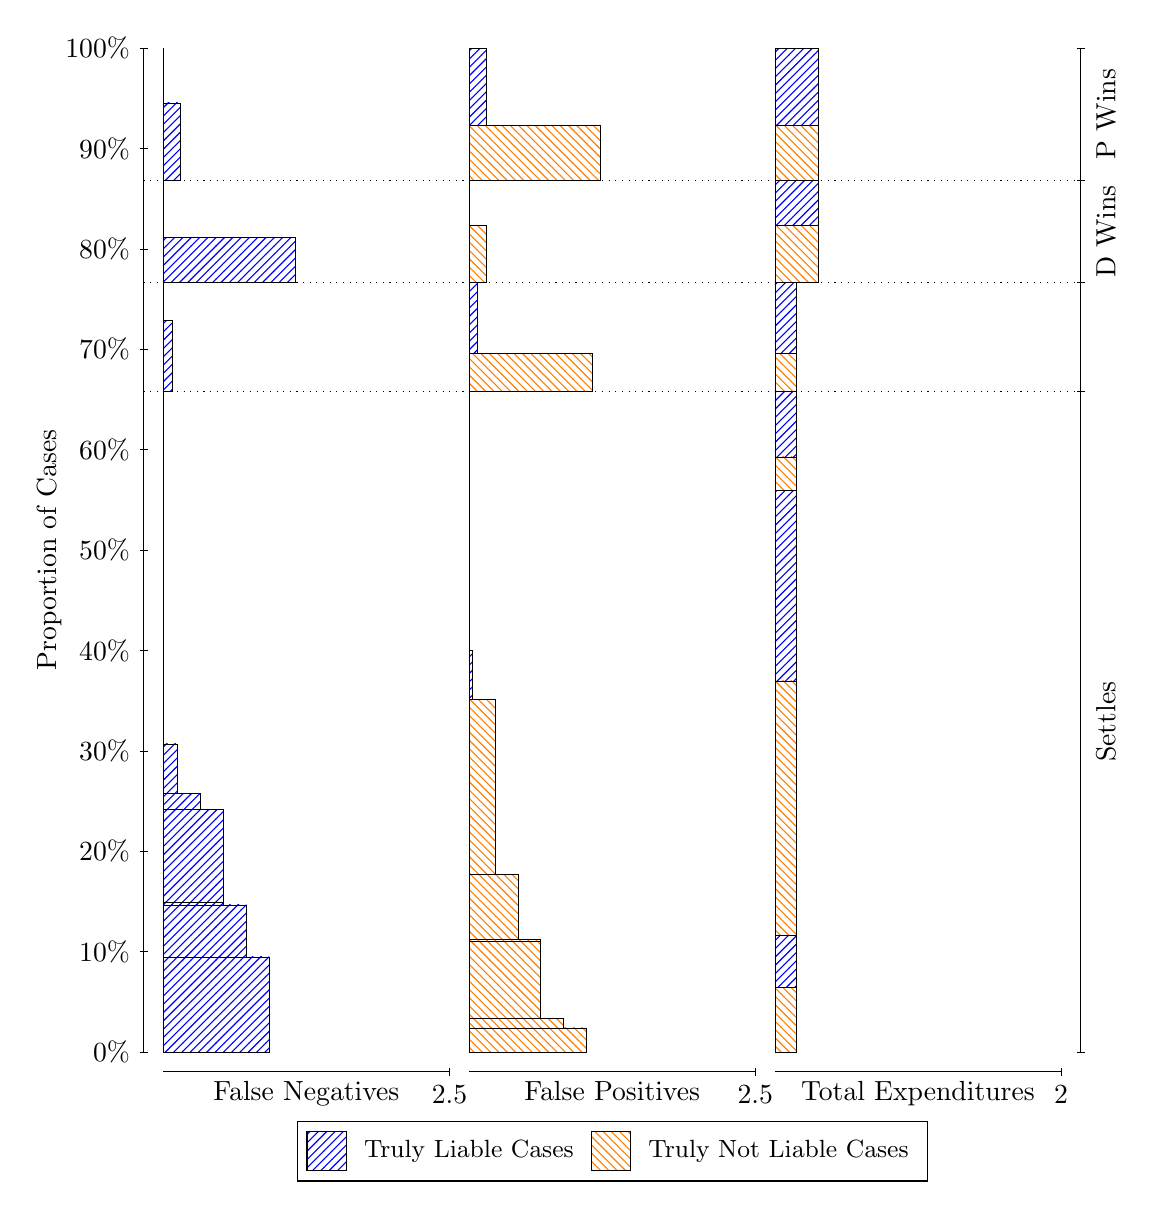
\begin{tikzpicture}
\draw[black, very thin] (1.5,1.75) -- (1.5,14.5);
\node[rotate=90, text=black, anchor=center] at (0.3, 8.125) {Proportion of Cases};
\draw[black, very thin] (1.45,1.75) -- (1.55,1.75);
\node[text=black, anchor=east] at (1.45, 1.75) {0\%};
\draw[black, very thin] (1.45,3.025) -- (1.55,3.025);
\node[text=black, anchor=east] at (1.45, 3.025) {10\%};
\draw[black, very thin] (1.45,4.3) -- (1.55,4.3);
\node[text=black, anchor=east] at (1.45, 4.3) {20\%};
\draw[black, very thin] (1.45,5.575) -- (1.55,5.575);
\node[text=black, anchor=east] at (1.45, 5.575) {30\%};
\draw[black, very thin] (1.45,6.85) -- (1.55,6.85);
\node[text=black, anchor=east] at (1.45, 6.85) {40\%};
\draw[black, very thin] (1.45,8.125) -- (1.55,8.125);
\node[text=black, anchor=east] at (1.45, 8.125) {50\%};
\draw[black, very thin] (1.45,9.4) -- (1.55,9.4);
\node[text=black, anchor=east] at (1.45, 9.4) {60\%};
\draw[black, very thin] (1.45,10.675) -- (1.55,10.675);
\node[text=black, anchor=east] at (1.45, 10.675) {70\%};
\draw[black, very thin] (1.45,11.95) -- (1.55,11.95);
\node[text=black, anchor=east] at (1.45, 11.95) {80\%};
\draw[black, very thin] (1.45,13.225) -- (1.55,13.225);
\node[text=black, anchor=east] at (1.45, 13.225) {90\%};
\draw[black, very thin] (1.45,14.5) -- (1.55,14.5);
\node[text=black, anchor=east] at (1.45, 14.5) {100\%};

\draw[black, very thin] (13.4,1.75) -- (13.4,14.5);
\draw[black, very thin] (13.35,1.75) -- (13.45,1.75);
\node[anchor=west] at (13.35, 1.75) {};
\draw[black, very thin] (13.35,10.139) -- (13.45,10.139);
\node[anchor=west] at (13.35, 10.139) {};
\draw[black, very thin] (13.35,11.519) -- (13.45,11.519);
\node[anchor=west] at (13.35, 11.519) {};
\draw[black, very thin] (13.35,12.821) -- (13.45,12.821);
\node[anchor=west] at (13.35, 12.821) {};
\draw[black, very thin] (13.35,14.5) -- (13.45,14.5);
\node[anchor=west] at (13.35, 14.5) {};

\draw[black, very thin, pattern color=blue, pattern=north east lines] (1.75,1.75) rectangle (3.0943,2.9576);
\draw[black, very thin, pattern color=blue, pattern=north east lines] (1.75,2.9576) rectangle (2.8037,3.6185);
\draw[black, very thin, pattern color=blue, pattern=north east lines] (1.75,3.6185) rectangle (2.513,3.6528);
\draw[black, very thin, pattern color=blue, pattern=north east lines] (1.75,3.6528) rectangle (2.513,4.8329);
\draw[black, very thin, pattern color=blue, pattern=north east lines] (1.75,4.8329) rectangle (2.2223,5.0336);
\draw[black, very thin, pattern color=blue, pattern=north east lines] (1.75,5.0336) rectangle (1.9317,5.6632);
\draw[black, very thin, pattern color=orange, pattern=north west lines] (1.75,5.6632) rectangle (1.75,10.139);
\draw[black, very thin, pattern color=blue, pattern=north east lines] (1.75,10.139) rectangle (1.859,11.04);
\draw[black, very thin, pattern color=orange, pattern=north west lines] (1.75,11.04) rectangle (1.75,11.519);
\draw[black, very thin, pattern color=blue, pattern=north east lines] (1.75,11.519) rectangle (3.4213,12.097);
\draw[black, very thin, pattern color=orange, pattern=north west lines] (1.75,12.097) rectangle (1.75,12.821);
\draw[black, very thin, pattern color=blue, pattern=north east lines] (1.75,12.821) rectangle (1.968,13.804);
\draw[black, very thin, pattern color=orange, pattern=north west lines] (1.75,13.804) rectangle (1.75,14.5);
\draw[black, very thin, pattern color=orange, pattern=north west lines] (5.6333,1.75) rectangle (7.123,2.0554);
\draw[black, very thin, pattern color=orange, pattern=north west lines] (5.6333,2.0554) rectangle (6.8323,2.1738);
\draw[black, very thin, pattern color=orange, pattern=north west lines] (5.6333,2.1738) rectangle (6.5417,3.1538);
\draw[black, very thin, pattern color=orange, pattern=north west lines] (5.6333,3.1538) rectangle (6.5417,3.1809);
\draw[black, very thin, pattern color=orange, pattern=north west lines] (5.6333,3.1809) rectangle (6.251,4.0026);
\draw[black, very thin, pattern color=orange, pattern=north west lines] (5.6333,4.0026) rectangle (5.9603,6.2259);
\draw[black, very thin, pattern color=blue, pattern=north east lines] (5.6333,6.2259) rectangle (5.6697,6.8555);
\draw[black, very thin, pattern color=blue, pattern=north east lines] (5.6333,6.8555) rectangle (5.6333,10.139);
\draw[black, very thin, pattern color=orange, pattern=north west lines] (5.6333,10.139) rectangle (7.1957,10.618);
\draw[black, very thin, pattern color=blue, pattern=north east lines] (5.6333,10.618) rectangle (5.7423,11.519);
\draw[black, very thin, pattern color=orange, pattern=north west lines] (5.6333,11.519) rectangle (5.8513,12.243);
\draw[black, very thin, pattern color=blue, pattern=north east lines] (5.6333,12.243) rectangle (5.6333,12.821);
\draw[black, very thin, pattern color=orange, pattern=north west lines] (5.6333,12.821) rectangle (7.3047,13.518);
\draw[black, very thin, pattern color=blue, pattern=north east lines] (5.6333,13.518) rectangle (5.8513,14.5);
\draw[black, very thin, pattern color=orange, pattern=north west lines] (9.5167,1.75) rectangle (9.7892,2.5716);
\draw[black, very thin, pattern color=blue, pattern=north east lines] (9.5167,2.5716) rectangle (9.7892,3.2326);
\draw[black, very thin, pattern color=orange, pattern=north west lines] (9.5167,3.2326) rectangle (9.7892,6.4631);
\draw[black, very thin, pattern color=blue, pattern=north east lines] (9.5167,6.4631) rectangle (9.7892,8.8851);
\draw[black, very thin, pattern color=orange, pattern=north west lines] (9.5167,8.8851) rectangle (9.7892,9.3088);
\draw[black, very thin, pattern color=blue, pattern=north east lines] (9.5167,9.3088) rectangle (9.7892,10.139);
\draw[black, very thin, pattern color=orange, pattern=north west lines] (9.5167,10.139) rectangle (9.7892,10.618);
\draw[black, very thin, pattern color=blue, pattern=north east lines] (9.5167,10.618) rectangle (9.7892,11.519);
\draw[black, very thin, pattern color=orange, pattern=north west lines] (9.5167,11.519) rectangle (10.062,12.243);
\draw[black, very thin, pattern color=blue, pattern=north east lines] (9.5167,12.243) rectangle (10.062,12.821);
\draw[black, very thin, pattern color=orange, pattern=north west lines] (9.5167,12.821) rectangle (10.062,13.518);
\draw[black, very thin, pattern color=blue, pattern=north east lines] (9.5167,13.518) rectangle (10.062,14.5);
\draw[black, dotted] (1.5,10.139) -- (13.4,10.139);
\draw[black, dotted] (1.5,11.519) -- (13.4,11.519);
\draw[black, dotted] (1.5,12.821) -- (13.4,12.821);
\draw[black, very thin] (1.75,1.5) -- (5.3833,1.5);
\node[text=black, anchor=north] at (3.5667, 1.5) {False Negatives};
\draw[black, very thin] (5.3833,1.45) -- (5.3833,1.55);
\node[text=black, anchor=north] at (5.3833, 1.45) {2.5};

\draw[black, very thin] (5.6333,1.5) -- (9.2667,1.5);
\node[text=black, anchor=north] at (7.45, 1.5) {False Positives};
\draw[black, very thin] (9.2667,1.45) -- (9.2667,1.55);
\node[text=black, anchor=north] at (9.2667, 1.45) {2.5};

\draw[black, very thin] (9.5167,1.5) -- (13.15,1.5);
\node[text=black, anchor=north] at (11.333, 1.5) {Total Expenditures};
\draw[black, very thin] (13.15,1.45) -- (13.15,1.55);
\node[text=black, anchor=north] at (13.15, 1.45) {2};

\node[text=black, centered, rotate=90] at (13.72, 5.9446) {Settles};

\node[text=black, centered, rotate=90] at (13.72, 12.17) {D Wins};
\node[text=black, centered, rotate=90] at (13.72, 13.661) {P Wins};

\draw (7.449999999999999,1.5) node[draw=none] (baseCoordinate) {};
\begin{scope}[align=center]
        \matrix[scale=0.5, draw=black, below=0.5cm of baseCoordinate, nodes={draw}, column sep=0.1cm]{
            \node[rectangle, draw, minimum width=0.5cm, minimum height=0.5cm, pattern color=blue, pattern=north east lines] {}; &
            \node[draw=none, font=\small, text=black] (B) {Truly Liable Cases}; &
            \node[rectangle, draw, minimum width=0.5cm, minimum height=0.5cm, pattern color=orange, pattern=north west lines] {}; &
            \node[draw=none, font=\small, text=black] (B) {Truly Not Liable Cases}; \\
            };
\end{scope}

\end{tikzpicture}
\end{document}